\subsubsection{UC-24 Creazione classe}

\begin{itemize}
	\item Attori: Insegnante
	\item Precondizione: L'insegnante si trova nella vista principale dell'applicazione.
	\item Postcondizione: L'insegnante si trova nella vista di gestione della classe* creata.
	\item Scenario principale:
	\begin{enumerate}
		\item L'insegnante selezione l'opzione "aggiungi classe"
		\item L'insegnante assegna un nome alla classe
		\item L'insegnante assegna una descrizione alla classe
		\item L'insegnante conferma la creazione (UC-32)
	\end{enumerate}

\end{itemize}

\subsubsection{UC-25 Eliminare una classe}
\begin{itemize}
	\item Attori: Insegnante
	\item Precondizione: L'insegnante si trova nella vista di gestione di una propria classe;
	\item Postcondizione: L'insegnante elimina la classe dal sistema.
	\item Scenario principale:
	\begin{enumerate}
		\item l'insegnante clicca sul pulsante di eliminazione della classe.
		\item l'insegnante conferma l'eliminazione (UC-32)
	\end{enumerate}
\end{itemize}

\subsubsection{UC-26 Inserimento Alunni}
\begin{itemize}
	\item Attori: Insegnante
	\item Precondizione: L'insegnante si trova nella vista di gestione di una propria classe;
	\item Postcondizione: L'insegnante visualizza gli alunni inseriti.
	\item Scenario principale:
	\begin{enumerate}
		\item l'insegnante seleziona l'opzione di aggiunta
		\item l'insegnante indica gli studenti da aggiungere
		\item l'insegnante conferma l'inserimento (UC-32)
	\end{enumerate}
\end{itemize}

\subsubsection{UC-27 Assegnazione Esercizi}
\begin{itemize}
	\item Attori: Insegnante
	\item Precondizione: L'insegnante si trova nella vista di gestione di una propria classe;
	\item Postcondizione: L'insegnante assegna esercizi alla classe.
	\item Scenario principale:
	\begin{enumerate}
		\item l'insegnante seleziona la classe
		\item l'insegnante assegna esercizi alla classe
		\item l'insegnante conferma l'inserimento (UC-32)
	\end{enumerate}
\end{itemize}



\subsubsection{UC-28 Visualizzare i progressi di un alunno della classe}
\begin{itemize}
	\item Attori: Insegnante
	\item Precondizione: L'insegnante visualizza l'elenco degli alunni iscritti alla classe;
	\item Postcondizione: L'insegnante visualizza i progressi relativi allo studente selezionato.
	\item Scenario principale:
	\begin{enumerate}
		\item l'insegnante seleziona uno studente. 
	\end{enumerate}
\end{itemize}

\subsubsection{UC-29 Elimina alunno dalla classe}		
\begin{itemize}
	\item Attori: Insegnante
	\item Precondizione: L'insegnante visualizza la lista degli alunni della classe.
	\item Postcondizione: L'insegnante ha rimosso l'allievo dalla classe.
	\item Scenario principale:
	\begin{enumerate}
		\item L'insegnante seleziona l'allievo da rimuovere dalla classe.
		\item L'insegnante conferma l'eliminazione. (UC-32)
	\end{enumerate}		
\end{itemize}

\subsubsection{UC-30 Visualizza lista degli alunni iscritti nella classe}		
\begin{itemize}
	\item Attori: Insegnante
	\item Precondizione: L'insegnante si trova nella vista di gestione di una propria classe.
	\item Postcondizione: L'insegnante visualizza l'elenco degli alunni iscritti.
	\item Scenario principale:
	\begin{enumerate}
		\item L'insegnante seleziona la classe
		\item L'insegnante seleziona l'opzione "vedi alunni".
	\end{enumerate}		
\end{itemize}

\subsubsection{UC-31 Visualizza lista delle classi}		
\begin{itemize}
	\item Attori: Insegnante, Allievo.
	\item Precondizione: L'utente si trova nella vista principale del proprio profilo.
	\item Postcondizione: L'utente visualizza le classi che lo riguardano.
	\item Scenario principale:
	\begin{enumerate}
		\item L'utente seleziona l'opzione "vedi classi".
	\end{enumerate}		
\end{itemize}

\subsubsection{UC-32 Conferma operazione}		
\begin{itemize}
	\item Attori: Utente
	\item Precondizione: L'utente ha inviato una richiesta di completamento dell'operazione
	\item Postcondizione: L'operazione viene annullata o confermata
	\item Scenario principale:
	\begin{enumerate}
		\item L'utente visualizza un messaggio per la conferma dell'operazione
		\item L'utente seleziona l'opzione "Conferma" per completare l'operazione.
	\end{enumerate}		
	\item Estensioni
		\begin{itemize}
			\item 2.a Se l'utente seleziona "Annulla", l'operazione non viene completata.
		\end{itemize}
\end{itemize}

\begin{figure}[h]
	\centering
	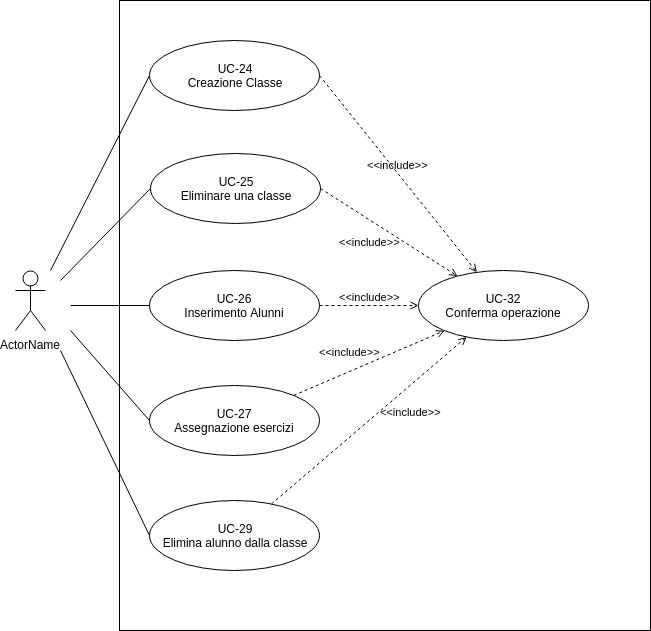
\includegraphics[scale=0.7]{images/UC-32.png}
\end{figure}
